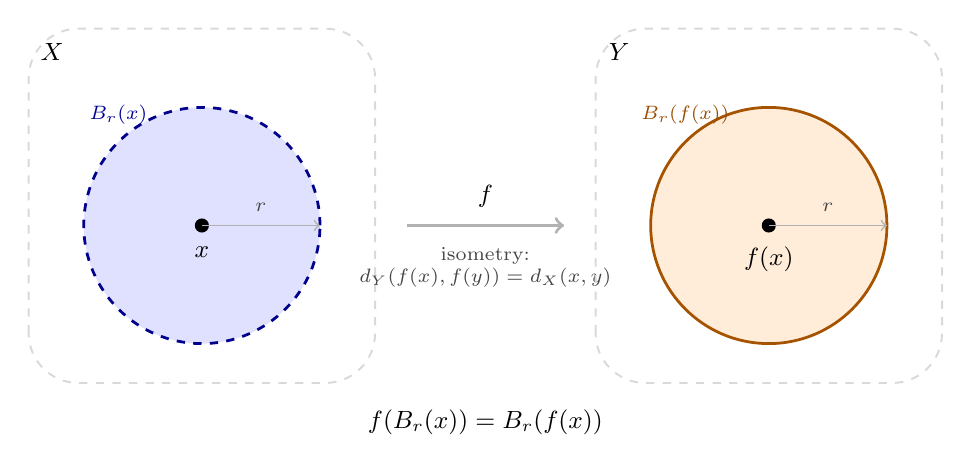
\begin{tikzpicture}[
  dot/.style={circle,fill,inner sep=1.8pt},
  lbl/.style={font=\small},
  sublbl/.style={font=\scriptsize,text=gray!55!black}
]

% ---- LEFT: space X ----
\begin{scope}[shift={(-3.6,0)}]
  % Background blob for X
  \draw[gray!30, line width=0.7pt, dashed, rounded corners=18pt]
    (-2.2,-2.0) rectangle (2.2,2.5);
  \node[lbl,font=\small\itshape] at (-1.9,2.2) {$X$};

  % Ball B_r(x)
  \fill[blue!12] (0,0) circle (1.5cm);
  \draw[blue!55!black, dashed, line width=1.0pt] (0,0) circle (1.5cm);

  % Centre x
  \node[dot,fill=black] at (0,0) {};
  \node[lbl,anchor=north] at (0,-0.15) {$x$};

  % Radius arrow
  \draw[gray!60,->,line width=0.6pt] (0,0) -- (1.5,0);
  \node[sublbl,anchor=south] at (0.75,0.05) {$r$};

  % Label
  \node[sublbl,text=blue!60!black,anchor=south]
    at ({-1.5*0.707},{1.5*0.707+0.1}) {$B_r(x)$};
\end{scope}

% ---- Arrow f in middle ----
\draw[->,line width=1.2pt,gray!60] (-1.0,0) -- (1.0,0);
\node[lbl,anchor=south] at (0,0.1) {$f$};
\node[sublbl,anchor=north,align=center] at (0,-0.15)
  {isometry:\\$d_Y(f(x),f(y))=d_X(x,y)$};

% ---- RIGHT: space Y ----
\begin{scope}[shift={(3.6,0)}]
  \draw[gray!30, line width=0.7pt, dashed, rounded corners=18pt]
    (-2.2,-2.0) rectangle (2.2,2.5);
  \node[lbl,font=\small\itshape] at (-1.9,2.2) {$Y$};

  % Ball B_r(f(x)) — same radius
  \fill[orange!15] (0,0) circle (1.5cm);
  \draw[orange!65!black, line width=1.0pt] (0,0) circle (1.5cm);

  % Centre f(x)
  \node[dot,fill=black] at (0,0) {};
  \node[lbl,anchor=north] at (0,-0.15) {$f(x)$};

  % Radius arrow
  \draw[gray!60,->,line width=0.6pt] (0,0) -- (1.5,0);
  \node[sublbl,anchor=south] at (0.75,0.05) {$r$};

  % Label
  \node[sublbl,text=orange!60!black,anchor=south]
    at ({-1.5*0.707},{1.5*0.707+0.1}) {$B_r(f(x))$};
\end{scope}

% Footer
\node[lbl,align=center] at (0,-2.5)
  {$f(B_r(x)) = B_r(f(x))$};
\end{tikzpicture}